% !TEX root = ../main.tex
\fancychapter{Related Work}%
\label{chap:related}
\cleardoublepage{}

\noindent
In this chapter, we expose and discuss numerical accuracy issues that arise when
performing computations with fixed-precision arithmetic.  We then proceed to
naming some precautions and steps in order to obtain practical solutions,
followed by a brief mention of some software libraries dedicated to overcoming
these issues through a series of exact algorithms and data structures.

We follow that by a comparative analysis of a set of \ac{GCS}-capable
programming tools along different dimensions, such as supported language
paradigm, native \ac{GCS} capabilities, 2D and 3D support.  Of those tools,
Eukleides, GeoSolver, and \acs{TikZ} \& \acs{PGF} are extensively discussed.

Similarly, we analyze \ac{AD} tools.  Some of them are integrated within
\ac{CAD} applications while others are standalone applications.  These tools and
their capabilities are summarized in \cref{tab:related.ad.summary}.
Furthermore, Dynamo and Grasshopper are expanded upon.

The chapter closes with small remarks on \acp{VPL}' poorer scalability with
increasing project complexity when compared to \acp{TPL}, showcasing the
\ac{RGC} as an example.

% !TEX root = ../../main.tex
\section{Robustness}%
\label{sec:related.robustness}

The correctness proofs of nearly all geometric algorithms presented in
theoretical papers assumes exact computation with real
numbers~\cite{CGAL:4.13:23LGK}.  However, floating-point numbers are represented
with fixed precision in computers, making them inexact, which leads to
inaccurate representations of the conceptual real number counterparts.  For
example, the rational number one-tenth ($\frac{1}{10}$) cannot be accurately
represented as a floating-point number, nor is it guaranteed to be truly equal
to another seemingly identical number.  Such comparisons must be performed
relying on tolerances, i.e., if $a$ and $b$ are two floating-point numbers, they
are considered \textit{the same} if $|a - b| \le \epsilon$ for a given tolerance
$\epsilon$.

As an example, consider the problem of finding the closest of two points
to the origin.  The distance between two points $P,Q \in \mathbb{R}^2$ can be
expressed by
%
\begin{equation}\label{eq:distance.2}
  d(P, Q) = \sqrt{(x_Q - x_P)^2 + (y_Q - y_P)^2}.
\end{equation}\equations{Euclidean distance between two points in $\mathbb{R}^2$}
%
Let $A,B \in \mathbb{R}^2$ be two arbitrary points, and $O \in \mathbb{R}^2$ the
origin.  To determine which point, $A$ or $B$, is closest to the origin $O$, we
compare the former's distances to the latter's.  That is, if
%
\[ 
  d(A, O) < d(B, O) 
\]
%
holds, $A$ is the closest to the origin.  Otherwise, they are either equidistant
or $B$ is closer.  However, applying the square root operation in the distance
computation is a step that will introduce errors.  Given that we are only
interested in comparing distances, and not use their actual value, we can,
instead, compare the squared distances.  As such, we avoid the square root, thus
improving robustness, and speeding up the process because the square root is a
computationally heavy operation.  \Citet{Mei:2014:NRGC} further discuss the
issues with numerical robustness in geometric computation, namely how they
arise, and propose practical solutions.

When used without care, fixed-precision arithmetic almost always leads to
unwanted results due to marginal error accumulation caused by rounding
(\textit{roundoff}), propagated throughout a series of calculations.  As seen
above, careful observations must be made before proceeding with computations as
simple as distance calculation.  To help solve this problem, more robust
numerical constructs and concepts can be used.  In particular, exact numbers,
such as rational numbers or arbitrary precision numbers. The latter, also known
as \textit{bignums}, allow arbitrary-precision arithmetic, capable of
representing numbers with virtually infinite precision with the drawback that
arithmetic operations are slower, however mitigating precision issues, providing
more accurate constructs and improving code robustness.

Several libraries already strive to implement robust geometric computation.  One
such example is \acf{CGAL}~\cite{CGAL:2018}.  \Ac{CGAL} is a comprehensive
library that employs an exact computation paradigm~\cite{Yap:1995:ECP},
producing correct results despite roundoff errors and properly handling
\textit{degenerate} situations (e.g., 3D points on a 2D plane), relying on
numbers with arbitrary precision to do so.  Moreover, other libraries, such as
\acs{LEDA}\label{acro:LEDA}~\cite{LEDA:2017,Mehlhorn:1989:LEDA}, and
CORE~\cite{Karamcheti:1999:CLRNGC} and its successor~\cite{Yu:2010:CORE2}, also
deal with robustness problems in geometric computation, offering simpler
interfaces when compared to \ac{CGAL}.  However, \ac{CGAL} arguably remains the
\textit{de facto} library for robust exact geometric computation.

% !TEX root = ../../main.tex
\subsection{Constraints in CAD}%
\label{sec:intro.constraints}

Parametric operations allow the user to create geometric objects that satisfy
certain constraints \emph{implicitly} imposed on the objects when the user
selects the operation they want.  \Acp{GC}, on the other hand, allow the
repositioning and scaling of objects so that they satisfy constraints the user
\emph{explicitly} imposed on them.

The abstract problem of \ac{GCS} consists of assigning coordinates to
constrained geometric objects such that the constraints they are subject to are
satisfied.  Otherwise, the solver should report no such assignment can be found.

One of the important features of a solver is its \emph{competence}, which is
related to the capability of reporting unsolvability: if no solution for the
problem exists and the solver is capable of reporting unsolvability, the solver
is deemed fully competent.  Since constraint solving is mostly an exponentially
complex problem~\cite{Rossi:2006:Handbook}, partial competence suffices as long
as decent solutions can be found in affordable time and space.

In the context of \ac{GCS}, it is also important that the \ac{GC} system does
not have too few or too many constraints.  Summarily, a system can either be 
\begin{enumerate*}[label= (\arabic*)]
  \item under-constrained, if the number of solutions is unbound due to lack of
  constraint coverage;
  \item over-constrained, if there are no solutions because of contradictions;
  or
  \item well-constrained, if the number of solutions is finite.
\end{enumerate*}

Some of the subjects approached here are briefed in~\cite{Hoffmann:2005:BCS}.
The following sections present and briefly discuss the most relevant approaches
to constraint solving.

\subsubsection{Graph-Based Approaches}%
\label{sec:intro.constraints.graph}

The problem is translated into a labeled \textit{constraint graph}, where
vertices are constrained geometric objects, and edges the constraints
themselves.  These became the dominant \ac{GCS} approaches.

\subsubsection{Logic-Based Approaches}%
\label{sec:intro.constraints.logic}

The constraint problem is translated into a set of geometric assertions and
axioms which is then transformed in such a way that specific solution steps are
made explicit by applying geometric reasoning.  The solver then takes a set of
construction steps and assigns coordinate values to the geometric entities.

\subsubsection{Algebraic Approaches}%
\label{sec:intro.constraints.algebraic}

The problem is translated into a system of equations, which is generally
nonlinear.  This approach's main advantage is its completeness and dimension
independence.  However, it is difficult to decompose the equation system into
subproblems, and a general, complete solution of algebraic equations is
inefficient.  Nonetheless, small algebraic systems tend to appear in the other
approaches and are routinely solved.

\subsubsection{Symbolic Methods}%
\label{sec:intro.constraints.symbolic}

Symbolic methods rely on general equation solvers that employ techniques to
triangularize equation systems~\cite{Chou:1988:IWMMTPG,Buchberger:1995:Grobner}
that emerge from employing an algebraic approach.  These methods can produce
generic solutions, but solvers are very slow and computation demands a lot of
space, usually requiring exponential running time~\cite{Durand:1998:SNTCS}.

\subsubsection{Numerical Methods}%
\label{sec:intro.constraints.numerical}

Among the oldest approaches to constraint solving, numerical methods solve large
systems of equations iteratively.  Methods like Newton iteration work properly
if a good approximation of the intended solution can be supplied and the system
is not ill-conditioned.  Alas, such methods may find only one solution, even in
cases where there are many, and may not allow the user to select the one they
are interested in.

\subsubsection{Theorem Proving}%
\label{sec:intro.constraints.proving}

\ac{GCS} can be seen as a subproblem of geometric theorem proving, but the
latter requires general techniques, therefore requiring much more complex
methods than those required by the former.

% !TEX root = ../../main.tex
\section{\acl{AD} Tools}
\label{sec:related.ad}

As discussed in \cref{sec:intro.ad}, \ac{AD} tools have been integrated into
several modern \ac{CAD} and \ac{BIM} applications; tools that use \acp{TPL},
\acp{VPL}, or even a mixture of both approaches.

Other tools, like OpenJSCAD and ImplicitCAD, are standalone \ac{CAD} software
hosted on the web.  Being cloud-based is advantageous in many fronts: it is
inherently portable, removes the additional typical installation steps required
for desktop applications.  Alas, being relatively new, they are lacking features
in comparison to the immense feature-set of applications such as AutoCAD.

\Cref{tab:related.ad.summary} succinctly summarizes a list of \ac{CAD} software
that includes the capability of designing resorting to the usage of a
programming language, as well as other \ac{AD} software and tools that live
detached from existing software.  From there, Dynamo and Grasshopper are further
comparatively discussed, being relatively similar tools, however integrated
within \ac{CAD}/\ac{BIM} software designed for performing different specific
tasks.  Moreover, both include \ac{TPL} and \ac{VPL} support in different forms.

\begin{table}[htbp]
  \begin{tabularx}{\textwidth}{|*{4}{c|}X|}
    \hline
    \textbf{Application} & \textbf{Tool} & \textbf{\acs{TPL}}
      & \textbf{\acs{VPL}} & \textbf{Note}\\
    \hline
    \hline
    \multirow{5}{*}{AutoCAD \cite{Autodesk:1982:AutoCAD}}
      & \multirow{2}{*}{.NET \acs{API}\label{acro:API}}
      & \multirow{2}{*}{\checkmark} & \multirow{2}{*}{\xmark}
      & \multirow{2}{*}{\parbox{\linewidth}{
        Powerful, but very verbose; C\# \& VB.NET}}\\
      &&&& \\ \cline{2-5}
      & \multirow{2}{*}{\parbox{7em}{\centering ActiveX Automation}}
        & \multirow{2}{*}{\checkmark} & \multirow{2}{*}{\xmark}
        & \multirow{2}{*}{\parbox{\linewidth}{
          Deprecated, bundled separately; \acs{VBA}\label{acro:VBA}}}\\
      &&&& \\ \cline{2-5}
      & Visual LISP & \checkmark & \xmark & \acs{IDE}\label{acro:IDE};
        AutoLISP extension\\
    \hline
    Dynamo Studio
      & \multirow{2}{*}{Dynamo \cite{Keough:2012:Dynamo}}
      & \multirow{2}{*}{\checkmark} & \multirow{2}{*}{\checkmark}
      & \multirow{2}{*}{\parbox{\linewidth}{%
        Data flow paradigm; Associative programming support through
        DesignScript}}\\\cline{1-1}
    Revit \cite{RevitTechCorp:2002:Revit} &&&&\\
    \hline
    ArchiCAD \cite{Graphisoft:2018:ArchiCAD}
      & \multirow{2}{*}{Grasshopper \cite{Rutten:2018:Grasshopper}}
      & \multirow{2}{*}{\checkmark} & \multirow{2}{*}{\checkmark}
      & \multirow{2}{*}{\parbox{\linewidth}{%
        Data flow paradigm; Rhino \acs{SDK} access, C\# \& VB.NET}}\\\cline{1-1}
    \multirow{4}{*}{Rhinoceros3D \cite{McNeel:2018:Rhinoceros3D}}
      &&&& \\ \cline{2-5}
      & \multirow{2}{*}{Python Scripting} & \multirow{2}{*}{\checkmark}
        & \multirow{2}{*}{\xmark}
        & \multirow{2}{*}{\parbox{\linewidth}{%
          Simple language; Create custom Grasshopper components}}\\
      &&&&\\\cline{2-5}
      & RhinoScript & \checkmark & \xmark & VBScript based\\
    \hline
    \multirow{5}{*}{\texttt{Standalone$^\dag$}}
      & ImplicitCAD \cite{Longtin:2018:ImplicitCAD}
        & \checkmark & \xmark & Web hosted; OpenSCAD inspired\\\cline{2-5}
      & OpenJSCAD \cite{Mueller:2019:OpenJSCAD}
        & \checkmark & \xmark & Web hosted; JavaScript\\\cline{2-5}
      & OpenSCAD \cite{Kintel:2019:OpenSCAD}
        & \checkmark & \xmark & Solid 3D models; Simple \acs{DSL}\label{acro:DSL}\\\cline{2-5}
      & \multirow{2}{*}{Rosetta \cite{Leitao:2011:PGDCAD}}
        & \multirow{2}{*}{\checkmark} & \multirow{2}{*}{\xmark}
        & \multirow{2}{*}{\parbox{\linewidth}{%
          Portable tool; Multiple front- and back-end support}}\\
      &&&&\\
    \hline
  \end{tabularx}
  \scriptsize
  $^\dag$These tools are standalone software, i.e., not directly integrated into
  any specific \ac{CAD} application.
  \caption[Table of programmatic \acs{CAD}/\acs{BIM} and \acs{AD} software]{%
    \ac{CAD}/\ac{BIM} software with programmatic capabilities and \ac{AD}
    software/tools.  Added notes per tool shortly outline deemed significant
    characteristics.}
  \label{tab:related.ad.summary}
\end{table}

\subsection{Dynamo}
\label{sec:related.ad.dynamo}

An open source \ac{AD} tool available as a plug-in for Revit or by itself within
Dynamo Studio, Dynamo extends \ac{BIM} with the data and logic environment of a
graphical algorithm editor \cite{Keough:2012:Dynamo}.  Dynamo can be used
through both a \ac{VPL} and a \ac{TPL}, showcased in
\cref{fig:related.ad.dynamo.node2code}.

\begin{figure}[htbp]
  \includegraphics[width=\textwidth]{fig/dynamo-node-to-code}
  {\scriptsize
  Source: \url{http://primer.dynamobim.org/en/07_Code-Block/7-2_Design-Script-syntax.html}
  (Jan 2019)}
  \caption[Dynamo's visual interface with node to code translation]{%
    Showcase of Dynamo's visual interface containing a workflow that produces
    the model on the top left.  The figure also shows Dynamo's capability of
    converting a the workflow to a single DesignScript code block.}
  \label{fig:related.ad.dynamo.node2code}
\end{figure}

In its visual form, Dynamo offers a wide variety of functions, called nodes,
most of them capable of generating an even wider variety of geometry through
node combination, wiring one's outputs to another's inputs, and resorting to
pre-defined mutable parameters which can serve as some of the nodes' initial
inputs.  The workflow itself is the final product: a visual program, usually
designed to execute a specific task.  Dynamo further allows extension through the
creation of custom nodes which can be shared as packages.

One of the nodes in Dynamo, aptly named code block, allows the usage of a
\ac{TPL}; a language called DesignScript.  Originally developed my Robert Aish
\cite{Aish:2011:DesignScript}, DesignScript is a multi-paradigm domain-specific
language and is the programming language at the core of Dynamo itself.  So much
so that entire workflows can be reduced to one code block (see
\Cref{fig:related.ad.dynamo.node2code}).

DesignScript is an associative language, which maintains a graph of dependencies
with variables.  Executing a script will effectively propagate the variables'
values accordingly.  By default, code blocks in Dynamo follow an associative
paradigm.  The user can, however, switch to an imperative paradigm approach
instead effortlessly if needed.

This \textit{change-propagation} mechanism in DesignScript, consequently present
in Dynamo, makes Dynamo a great tool for dealing with constraints.  However,
most users might not fully exercise DesignScript's associative capabilities and
instead approach the problem with the mindset of an imperative programming
paradigm given its overwhelming presence in and adoption by major well-known
\acp{TPL}.

\subsection{Grasshopper}
\label{sec:related.ad.grasshopper}

Grasshopper is a graphical algorithm editor tightly integrated with
Rhinoceros3D, destined for designers who are exploring generative algorithms
\cite{Rutten:2018:Grasshopper}.  In spite of tight integration with Rhino, a
\ac{CAD} application, it is possible to use Grasshopper along with ArchiCAD
\cite{Graphisoft:2018:ArchiCAD,Graphisoft:2018:RGACAD}, a \ac{BIM} tool.
\Cref{fig:related.ad.grasshopper.islamic-pattern} shows a simple example of a
Grasshopper workflow.

\todo[inline]{Replace example with Rythmic Gynmastics Center, Moscow, Russia}

\begin{figure}[htbp]
  \includegraphics[width=\textwidth]{fig/grasshopper-islamic-pattern}
  {\scriptsize
  Source: \url{https://www.grasshopper3d.com/photo/islamic-pattern-parakeet}
  (Jan 2019)}
  \caption[Islamic Pattern in Grasshopper using Parakeet]{
    Islamic Pattern, by Esmaeil Mottaghi.  On top is the Grasshopper workflow to
    produce the pattern below it, aided by Parakeet
    \cite{Esmaeil:2018:Parakeet}.}
  \label{fig:related.ad.grasshopper.islamic-pattern}
\end{figure}

It is a closed-source product, designed by David Rutten and developed by McNeel
and Associates, Rhino's developers.  Its \ac{VPL} is as simple to use as
Dynamo's, which is crucial for users who are not familiar with programming using
a \ac{TPL}.  Nonetheless, it offers a \ac{TPL} alternative by way of custom
programmatic components.  Using C\# or VB.NET, the user can create custom code
components with access to Rhino's \ac{SDK} and OpenNURBS
\cite{Lear:2018:openNURBS} within Rhino.  Alternatively, through GhPython
\cite{Giulio:2017:GhPython}, the user can also write Python code.  Unlike
DesignScript, Python and the .NET languages don't support an associative
programming model.

Functions in Grasshopper are called components and work just like Dynamo's
nodes; a wide variety of them exist, most of them capable of producing geometry,
and they are composable, generating a workflow destined to accomplish a specific
task.

Both Dynamo and Grasshopper's visual approach suffer from the unproportionate
scalability between the code and the respective model's complexity
\cite{Leitao:2014:PESLGD}.  Sophisticated modelling workflows tend to become
difficult to properly represent, and harder for a human to efficiently interpret
when compared to a textual approach.  This disadvantage, however, is mitigated
with their respective \ac{TPL} alternatives.

\subsection{Visual Programming Scalability}%
\label{sec:related.ad.vpl-scalability}

Both Dynamo and Grasshopper's visual approach suffer from the disproportionate
scalability between the code and the respective model's
complexity~\cite{Leitao:2013:PESLGD}.  Sophisticated modeling workflows tend to
become difficult to properly represent, and harder for a human to efficiently
interpret when compared to a textual approach.

As an example, consider the Irina Viner-Usmanova \ac{RGC}, a project developed
by TPO Pride\footnote{\url{http://prideproject.pro} (July 2, 2021)} over the
span of three years, from 2016 to 2019.  The \ac{RGC}, built in Moscow's
Luzhniki Stadium, is an arena that houses training sessions and competitions
while also comprising several other premises.
\Cref{fig:related.ad.vpl-scalability.rgc} depicts an outside view of the
\ac{RGC} and its prominent overarching roof covering.  The roof covering was
designed using a combination of Rhino3D and Grasshopper.  Grasshopper was used
from a conceptual stage all the way through to production of construction
drawings.

\begin{figure}[htb]
  \includegraphics[width=\textwidth]{fig/rgc}\\
  {\scriptsize
  Source: \url{https://www.grasshopper3d.com/photo/rhythmic-gymnastics-center-moscow-russia-5}
  (Jul 2021)
  }
  \caption[\acl{RGC} in the Luzhniki Complex]{
    Irina Viner-Usmanova \ac{RGC} in the Luzhniki Complex, Moscow, Russia.  The
    roof covering was designed using Rhino/Grasshopper.}%
  \label{fig:related.ad.vpl-scalability.rgc}
\end{figure}

Developing a roof covering with such a contour lends itself well to \ac{AD}
since it resembles a sine wave whose amplitude is progressively dampened along
the length of the building.  Such a shape can be easily described through a
relatively simple mathematical function to obtain the general wave's shape.
With parametrization in mind, one could then easily fluctuate input variables in
order to achieve different variations of the roof covering's shape, e.g.,
varying the underlying wave's frequency, amplitude, or dampening rate.

Such complex \ac{AD} projects hide equally, if not more, complex corresponding
programs.  The final Grasshopper definition of the \ac{RGC} roof's covering can
be seen in \cref{fig:related.ad.vpl-scalability.rgc-gh}.  This further
reinforces the statement that complex workflows become exponentially difficult
to comprehend due to the added dimensionality of the constructs used in
\acp{VPL}.  This disadvantage, however, is mitigated with their respective
\ac{TPL} alternatives which, despite project complexity, scale relatively better
than \acp{VPL} as the former rely on text, which is one-dimensional, while the
latter rely on boxes and interconnecting wires, which are two-dimensional.

\begin{figure}[htb]
  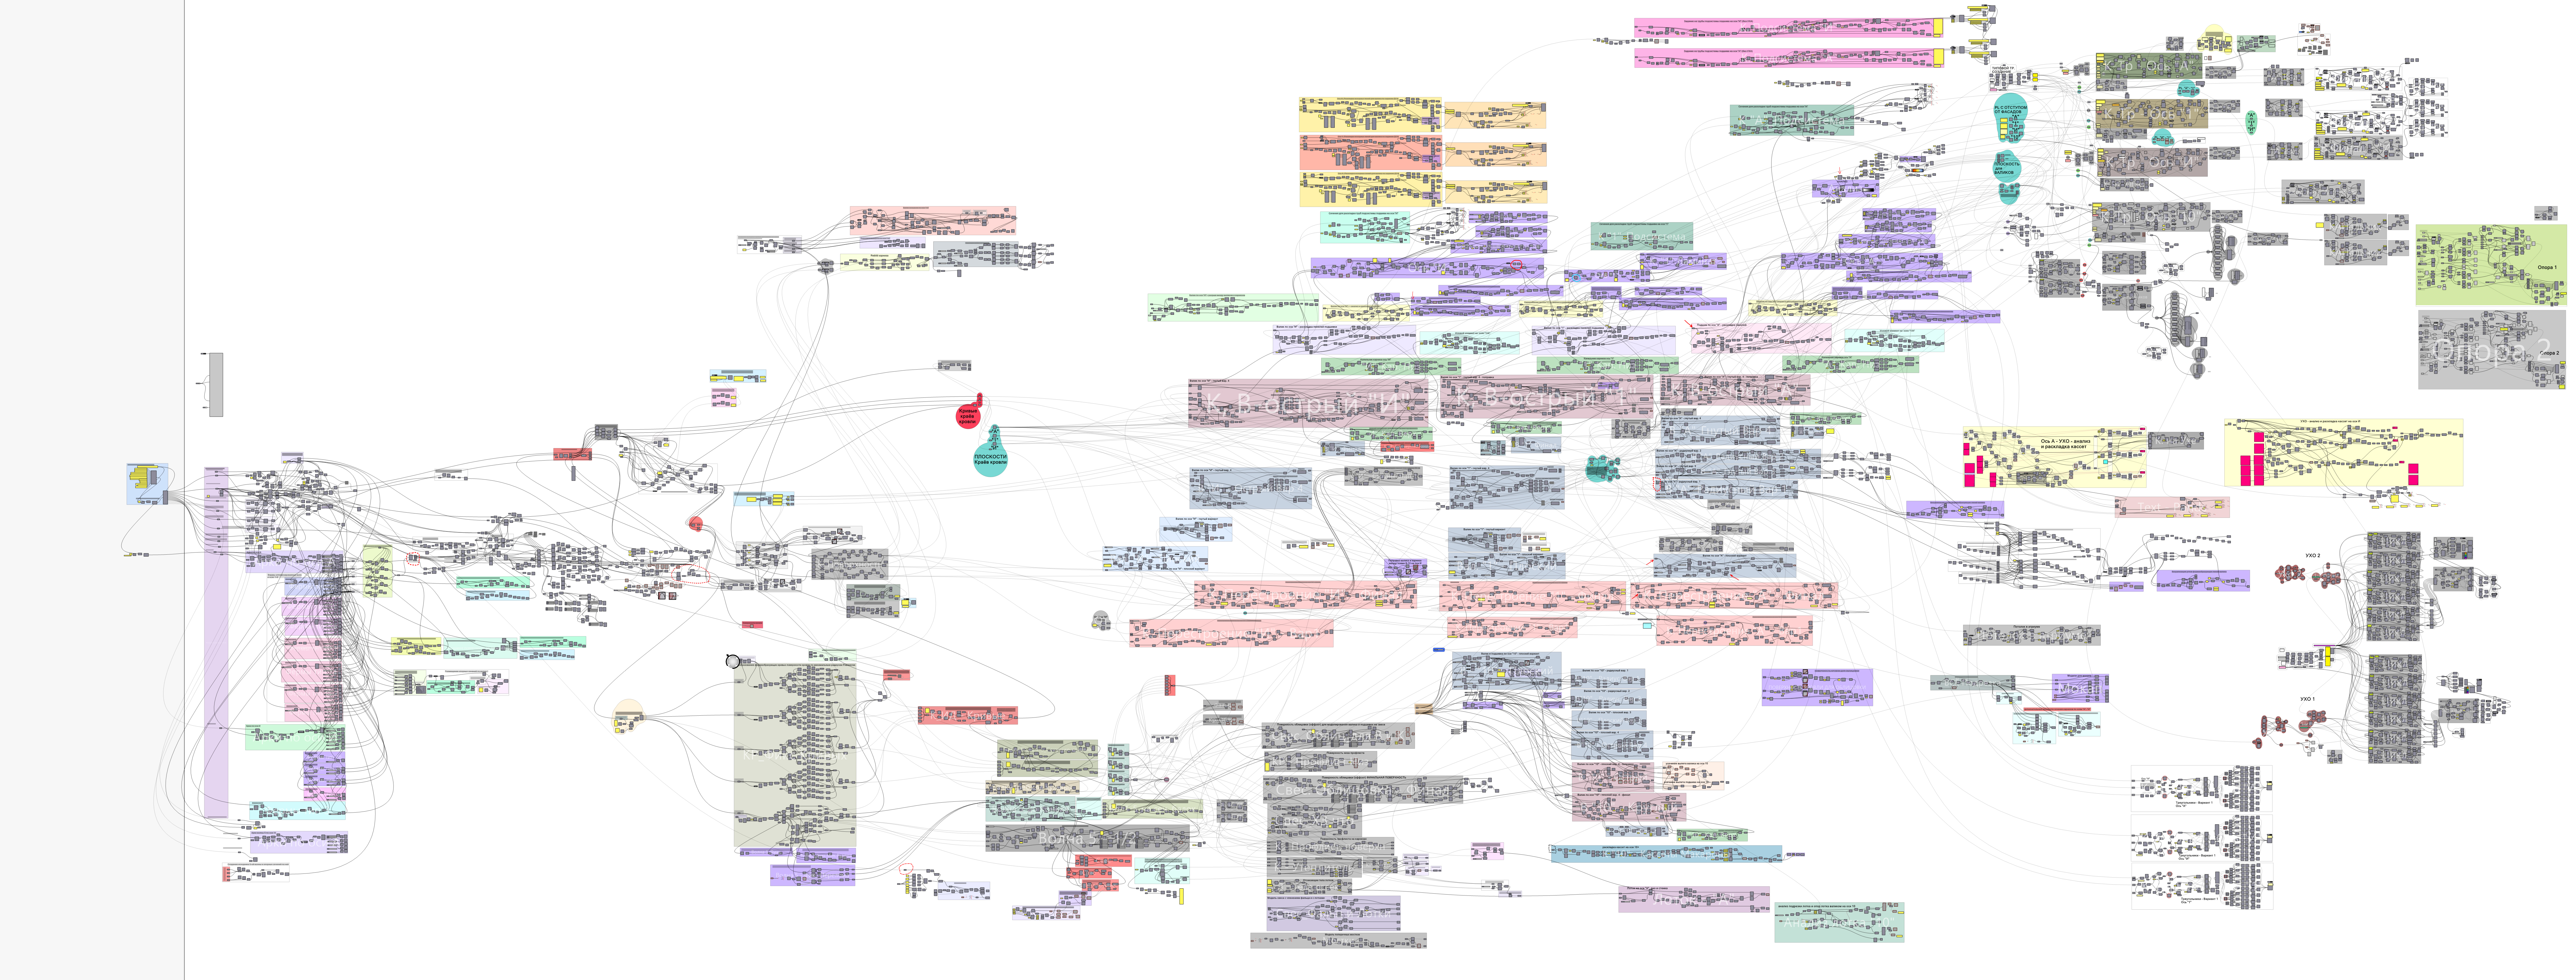
\includegraphics[width=\linewidth]{fig/rgc-gh}\\
  {\scriptsize
  Source: \url{https://www.grasshopper3d.com/photo/final-definition} (Jul 2021)
  }
  \caption[Grasshopper definition of the \acl{RGC} roof covering]{
    Final Grasshopper definition of the Irina Viner-Usmanova \ac{RGC} roof
    covering.}%
  \label{fig:related.ad.vpl-scalability.rgc-gh}
\end{figure}

